% This is samplepaper.tex, a sample chapter demonstrating the
% LLNCS macro package for Springer Computer Science proceedings;
% Version 2.20 of 2017/10/04
%
\documentclass[runningheads]{llncs}

\usepackage[T1]{fontenc}
\usepackage[utf8]{inputenc}
\usepackage{graphicx}
\usepackage{listings}
\usepackage{wrapfig}
\usepackage{hyperref}
\usepackage{stmaryrd}

\DeclareUnicodeCharacter{21D2}{$\Rightarrow$}
\DeclareUnicodeCharacter{2227}{$\land$}
\DeclareUnicodeCharacter{2228}{$\lor$}
\DeclareUnicodeCharacter{2260}{$\neq$}
\DeclareUnicodeCharacter{2265}{$\geq$}
\DeclareUnicodeCharacter{2264}{$\leq$}
\DeclareUnicodeCharacter{27F9}{$\Longrightarrow$}
\DeclareUnicodeCharacter{2987}{$\llparenthesis$}
\DeclareUnicodeCharacter{2988}{$\rrparenthesis$}

% redefined to give listings in tt font
\renewcommand{\lstinline}[1]{\texttt{#1}}

% Used for displaying a sample figure. If possible, figure files should
% be included in EPS format.
%
% If you use the hyperref package, please uncomment the following line
% to display URLs in blue roman font according to Springer's eBook style:
% \renewcommand\UrlFont{\color{blue}\rmfamily}

\begin{document}
%
\title{Marlowe: implementing and analysing financial contracts on blockchain}%\thanks{Supported by IOHK.}}
%
%\titlerunning{Abbreviated paper title}
% If the paper title is too long for the running head, you can set
% an abbreviated paper title here
%
\author{
Pablo {Lamela Seijas}\inst{1} \and
Alexander Nemish\inst{1} \and \\
David Smith\inst{1} \and
Simon Thompson\inst{1,2}}%\orcidID{0000-0002-2350-301X}}
%
\authorrunning{P. Lamela Seijas, A. Nemish, et al.}

% First names are abbreviated in the running head.
% If there are more than two authors, 'et al.' is used.
%
\institute{IOHK, Hong Kong, 
\email{alexander.nemish@iohk.io, pablo.lamela@iohk.io, simon.thompson@iohk.io,~david.smith@tweag.io},  \and
School of Computing, University of Kent, UK, 
\email{s.j.thompson@kent.ac.uk}}
%
\maketitle              % typeset the header of the contribution

\vspace{-4mm}
\begin{abstract}
Marlowe is a DSL for financial contracts. We describe the implementation of Marlowe on the Cardano blockchain, and the Marlowe Playground web-based development and simulation environment.

Contracts in Marlowe can be exhaustively analysed prior to running them, thus providing strong guarantees to participants in the contract. The Marlowe system itself has been formally verified using the Isabelle theorem prover, establishing such properties as the conservation of money.

\keywords{Cardano \and DSL \and functional \and Haskell \and SMT \and static analysis}
\end{abstract}


\section{Introduction}

Marlowe\footnote{The complete Marlowe project, including semantics and implementation, is available at \url{https://github.com/input-output-hk/marlowe}.} is a domain-specific language (DSL) for implementing financial contracts on blockchain: our initial target is Cardano, but it could be implemented on many distributed ledgers (DLT platforms), including Ethereum. Marlowe is embedded in Haskell, allowing users selectively to use aspects of Haskell -- typically definitions of constants and simple functions -- to express contracts more readably and succinctly. Section \ref{sec:overview} gives an overview of the language, and the changes made to it since it was originally introduced in ~\cite{isola-marlowe}.

Marlowe is specified by a reference semantics for the language written in Haskell, and we can use that in a number of ways. We can interpret Marlowe contracts in Haskell itself, but we can also use that implementation, compiled into Plutus~\cite{PlutusPlatform}, to interpret Marlowe directly on the Cardano blockchain, see Section \ref{sec:implementation}. We can also execute the semantics -- translated into PureScript -- directly in a browser, to give an interactive simulation environment, see Section~\ref{sec:playground}.

Because Marlowe is a DSL, we are able to build special purpose tools and techniques to support it. Crucially in a financial environment, we are able to \emph{exhaustively analyse contracts} without executing them, so that we can, for instance, check whether any particular contract is able to make all the payments it should: in the case it is not, we get an explicit example of how it can fail. This analysis, reported in Section \ref{sec:static}, is built into the Marlowe Playground. Finally, we are able to use formal verification to prove properties of the implementation of Marlowe, including a guarantee that ``money in $=$ money out'' for all contracts; see Section~\ref{sec:verification}.

\section{Marlowe overview}
\label{sec:overview}

Since the first publication, we have revised the language design: this section gives a brief overview of the current (3.0) version of the language and its semantics.


\subsubsection*{The Marlowe model}

Contracts are built by putting together a small number of constructs that in combination can be used to describe many different kinds of financial contract.

Contracts in Marlowe run on a blockchain, but need to interact with the off-chain world. The parties to the contract, also called the participants, can engage in various actions: they can be asked to deposit money, or to make a choice between various alternatives. In some cases, any party will be able to trigger the contract just to notify it that some condition has become true (for example, a timeout has occurred).

The Marlowe model allows for a contract to control money in a number of disjoint accounts: this allows for more explicit control of how the money flows in the contract. Each account is owned by a particular party to the contract, and that party receives a refund of any remaining funds in the account when the contract is closed. %These accounts are local, in that they only exist as during the execution of the contract, and during that time they are only accessible by parties to the contract.

Marlowe contracts describe a series of steps, typically by describing the first step, together with another (sub-) contract that describes what to do next. For example, the contract \texttt{Pay a p v cont} says ``make a payment of \texttt{v} Lovelace to the party \texttt{p} from the account \texttt{a}, and then follow the contract \texttt{cont}''. We call \texttt{cont} the continuation of the contract.

In executing a contract, we need to keep track of the current contract: after making a step in the example above, the current contract would be \texttt{cont}. We also have to keep track of some other information, such as how much is held in each account: this information together is the state, which generally changes at each step. A step can also see an action taking place, such as money being deposited, or an effect being produced, e.g. a payment.
%Value on the blockchain resides in the UTxO, which are protected cryptographically by a private key held by the owner. These keys can be used to redeem the output, and so to use them as inputs to new transactions, which can be seen as spending the value in the inputs. Users typically keep track of their private keys, and the values attached to them, in a cryptographically-secure wallet.
It is through their wallets that users are able to interact with Marlowe contracts running on the blockchain, making deposits and receiving payments. %Note, however, that these are definitely off chain actions that need to be controlled by code running in the user's wallet: they cannot be made to happen by the Marlowe contract itself.

%\subsection{Executing a Marlowe contract}
%At each slot, a running Marlowe contract will receive a list of inputs in order. The contract is executed by evaluating it step by step until it cannot be changed any further without processing any input, a condition that we call being quiescent. The first input is then processed, and then the contract is single stepped again until quiescence, and this process is repeated until all the inputs are processed. At each step the current contact and the state will change, some input may be processed, and payments made.


\subsubsection*{Marlowe step by step}

Marlowe has five ways of building contracts, we call these \emph{contract constructs}. \emph{Contract constructs}, in turn, can also contain \emph{values}, \emph{observations} and \emph{actions}.

\paragraph{Values, observations and actions} are used to supply external information and inputs to a running contract to control how it will evolve.

\texttt{Value}s include some quantities that change with time, like the current slot number, the current balance of an account, and any choices that have already been made. % ; we call these volatile values. - PLS: this definition is no longer used
Values can be combined using addition, subtraction and negation.

\texttt{Observation}s are Boolean expressions that compare values, and can be combined using the standard Boolean operators. It is also possible to observe whether any choice has been made (for a particular identified choice). Observations will have a value at every step of execution.

\texttt{Action}s happen at particular points during execution and can be (i) depositing money, (ii) making a choice between various alternatives, or (iii) notifying the contract that a certain observation has become true.

\paragraph{Contract constructs} are the main building block of contracts, and there are five of them: four of these -- \texttt{Pay}, \texttt{Let}, \texttt{If} and \texttt{When} -- build a complex contract from simpler contracts, and the fifth, \texttt{Close}, is a simple contract. At each step of execution we will obtain a new state and continuation contract and, in some it is possible that effects, like payments and warnings, can be generated too.

\texttt{Pay}: A payment contract \texttt{Pay a p v cont} will make a payment of value \texttt{v} from the account \texttt{a} to a payee \texttt{p}, which will be one of the contract participants or another account in the contract. Warnings will be generated if the value \texttt{v} is not positive, or if there is not enough in the account to make the payment in full. In the first case, nothing will be transferred; in the later case, a partial payment (of all the money available) is made. The contract will continue as \texttt{cont}.

\texttt{Close}: A contract \texttt{Close} provides for the contract to be closed (or terminated). The only action that is performed is to refund the contents of each account to their respective owners. This is performed one account per step, but all accounts will be refunded in a single transaction. All contracts eventually reduce to \texttt{Close}.

%Before discussing other forms of contracts, we need to describe values, observations and actions.

\texttt{If}: The conditional \texttt{If obs cont1 cont2} will continue as \texttt{cont1} or \texttt{cont2}, depending on the Boolean value of the observation \texttt{obs} on execution.

\texttt{When}: This is the most complex constructor for contracts, with the form \texttt{When cases timeout cont}. It is a contract that is triggered on actions, which may or may not happen at any particular slot: the permitted actions and their consequences are described by \texttt{cases}.

The list \texttt{cases} contains a collection of cases of the form \texttt{Case ac co}, where \texttt{ac} is an action and \texttt{co} a continuation (another contract). When the action \texttt{ac} is performed, the state is updated accordingly and the contract will continue as described by \texttt{co}.

In order to make sure that the contract makes progress eventually, the contract \texttt{When cases timeout cont} will continue as \texttt{cont} as soon as any valid transaction is issued after the \texttt{timeout} (a slot number) is reached.

\texttt{Let}: A let contract \texttt{Let id val cont} causes the expression \texttt{val} to be evaluated, and stored with the name \texttt{id}. The contract then continues as \texttt{cont}.

%As well as allowing us to use abbreviations, this mechanism also means that we can capture and save volatile values that might be changing with time, e.g. the current price of oil, or the current slot number, at a particular point in the execution of the contract, to be used later on in contract execution.


%%% end overview



\section{Implementation of Marlowe on Cardano}
\label{sec:implementation}

Marlowe is specified by an executable semantics written in Haskell, but to make it usable in practice with financial contracts, it needs to be implemented on a blockchain. In this section, we explain how Marlowe is executed on the Cardano blockchain using an interpreter \footnote{The implementation is available at \url{https://github.com/input-output-hk/plutus/blob/0ca9af4f6614d591de7ebbe4dd759ce122d74efd/marlowe/src/Language/Marlowe/Semantics.hs}.} written in the Plutus programming language.

\subsection{Cardano and Plutus}

Cardano is a third-generation blockchain that solves the energy usage
issue by moving to an energy efficient \emph{Proof of Stake} protocol~\cite{Ouroboros-Genesis}.

Cardano aims to support smart contracs during its Shelley release in 2020.
Cardano smart contract platform is called \emph{Plutus}, and
it uses Haskell programming language to generate a form of $System F_{\omega}$,
called \emph{Plutus Core}, by extending GHC using its plugin
support~\cite[Section 13.3]{ghcusersguide}.

To implement Marlowe contracts, we use the PlutusTx compiler,
which compiles Haskell code into serialized \emph{Plutus Core} code,
to create a Cardano \emph{validator script} that ensures the correct execution of the contract.
This form of implementation relies on the extensions to the UTxO model described in~\cite{PlutusPlatform}.


\subsection{Extended UTxO}

Cardano is a UTxO-based (unspent transaction output) blockchain, similar to Bitcoin~\cite{sok}.
It extends the Bitcoin model by allowing transaction outputs to hold a \emph{Data Script}.
As the name suggests, this is  a serialised data value used to store and communicate a contract state.
This allows us to create complex multi-transactional contracts.
In a nutshell, the EUTxO model looks like this:

\begin{figure}[!h]
    \centering
    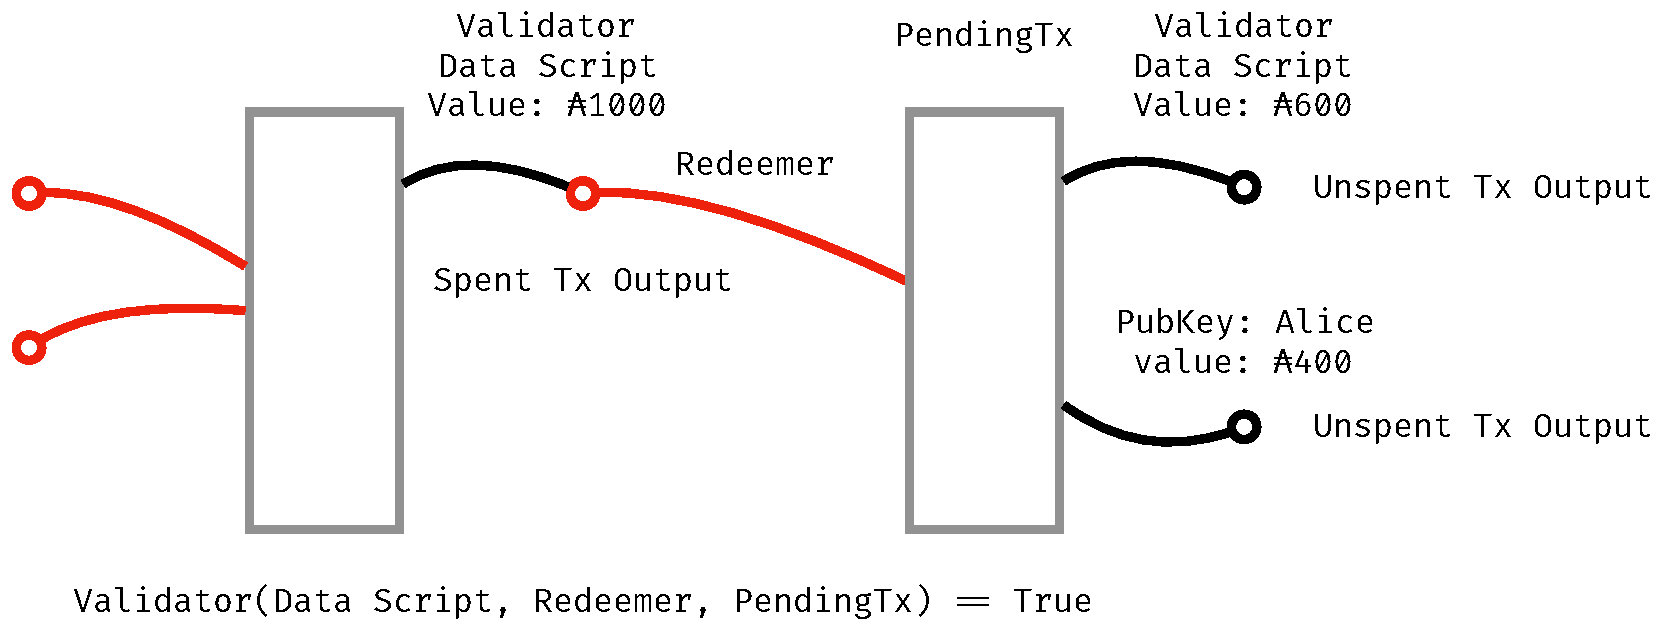
\includegraphics[width=4in]{figures/Marlowe3-Figure-1-crop.pdf}
    \caption{Cardano EUTx0 Model}
    \label{fig:eutxo}
\end{figure}

\noindent
where black circles represent \emph{unspent transaction outputs}, and red lines show \emph{transaction inputs}
that reference existing \emph{transaction outputs}.
Each transaction output contains a \emph{Value}, and is protected either by a \emph{public key},
or by a \emph{Validator}.

In order to spend an existing transaction output protected by a \emph{Validator},
one must create a transaction (a \emph{PendingTx}) that has an \emph{input} that references the transaction output,
and contains a \emph{Redeemer}, such that \texttt{Validator(Data Script, Redeemer, PendingTx)} evaluates to $True$.
A valid signature is required to spend a \emph{public key} transaction output.


\subsection{Design space}

There are several ways to implement Marlowe contracts on top of Plutus.
We could write a Marlowe to Plutus compiler that would convert
each Marlowe contract into a specific Plutus script.
Instead, we chose to implement a Marlowe interpreter as a single Plutus script.
This approach has a number of advantages:
\begin{itemize}
\item It is simple: having a single Plutus script that implements all Marlowe contracts
makes it easier to implement, review, and test what we have done.
\item Implementation is close to the semantics of Marlowe, as sketched above and in more detail in~\cite{isola-marlowe},
which makes it easier to validate.
\item The same implementation can be used for both on- and off-chain (wallet) execution of Marlowe code.
\item It facilitates client-side contract evaluation, where we reuse the same code
to do contract execution emulation in an IDE, and compile it to WASM/JavaScript on the client side,
e.g.\ in the Marlowe Playground.
\item Having a single interpreter for all (or a particular group of) Marlowe contracts allows us
  to monitor the blockchain for these contracts, if required.
\item Finally, Cardano nodes could potentially use an optimised interpreter (e.g:~native) just for Marlowe contracts, which would save processing time.
\end{itemize}

\noindent
Marlowe contract execution on the blockchain consists of a chain of transactions
where, at each stage, the remaining contract and its state are passed through the \emph{Data script},
and actions/inputs (i.e. \emph{choices} and \emph{money deposits}) are passed via the 
%SJT: is this right?
%AN: yes. [Input] is precisely the redeemer script. We could say that Value and SlotInterval are parts of PendingTx,
% but I think it's not that important here.
\emph{Redeemer}.
Each step in contract execution is a transaction that spends a Marlowe contract transaction output
by providing a valid input as \emph{Redeemer}, and produces a transaction output
with a the remaining Marlowe contract and the updated state.

We store the remaining contract in the \emph{Data script}, which makes it visible to everyone.
This simplifies contract reflection and retrospection.

\subsection{Contract lifecycle on the extended UTxO model}

As described above, the Marlowe interpreter is realised as a \emph{Validation script}.
We can divide the execution of a Marlowe Contract into two phases:
creation and execution.

\paragraph{Creation}

Contract creation is realised as a transaction
with at least one script output,
with the particular Marlowe contract in the data script, and protected by the Marlowe validator script.
Note that we do not place any restriction on the transaction inputs, which could use any other transaction
outputs, including other scripts. This gives this model optimal flexibility and composability.

\begin{verbatim}
data MarloweData = MarloweData {
    marloweState    :: State,
    marloweContract :: Contract
}
\end{verbatim}
\noindent
The contract has a state

\begin{verbatim}
data State = State { accounts    :: Map AccountId Ada
                   , choices     :: Map ChoiceId ChosenNum
                   , boundValues :: Map ValueId Integer
                   , minSlot     :: Slot }
\end{verbatim}

\noindent
where \texttt{accounts} maps account ids to their balances, \texttt{choices} stores user made choice values,
\texttt{boundValues} stores evaluated \texttt{Value}'s introduced by \texttt{Let} expressions,
and \texttt{minSlot} holds a minimal slot number that a contract has seen, to avoid `time travel to the past'.

\paragraph{Execution}

Marlowe contract execution consists of a chain of transactions,
where the remaining contract and state are passed through the \emph{data script},
and input actions (i.e. \texttt{choices}) are passed as \emph{redeemer scripts}.

Each execution step is a transaction that spends a Marlowe contract transaction output by providing
an expected input in a redeemer script,
and produces a transaction output with a Marlowe contract as continuation.

The Marlowe interpreter first validates the current contract state: i.e.\
we check that the contract locks at least as much as specified by the
contract balances (the \texttt{accounts} field in \texttt{State}),
and that balances are strictly positive.
\footnote{
Using the Isabelle proof assistant, we have formally verified that given a state with positive balances,
it is impossible for any possible contract and inputs to result in non-positive balances.
This is described in more detail in Section \ref{subsec:valid_state}.}

We then compute expected transaction outcomes for given inputs, such as:
contract continuation, new state, and payments.

\begin{verbatim}
expectedTxOutputs = computeTransaction txInput marloweState marloweContract
\end{verbatim}

\noindent
where

\begin{verbatim}
computeTransaction :: TransactionInput -> State -> Contract -> TransactionOutput

data TransactionInput = TransactionInput
    { txInterval :: SlotInterval
    , txInputs   :: [Input] }

data TransactionOutput =
    TransactionOutput
        { txOutWarnings :: [TransactionWarning]
        , txOutPayments :: [Payment]
        , txOutState    :: State
        , txOutContract :: Contract }
    | Error TransactionError
\end{verbatim}

\noindent
Given a list of \texttt{Input}'s from \emph{Redeemer}, the interpreter reduces a contract until it becomes quiescent: either it evaluates to \texttt{Close},
or it expects a user input in a \texttt{When} construct.
All \texttt{Pay, If, Let, Close} constructs are evaluated immediately.

The evaluation function returns a new contract state, contract continuation, a list of warnings (such as partial payments),
and a list of expected payments (i.e. one for each of the \texttt{Pay} constructs evaluated).

The on-chain \emph{Validator} code cannot generate transaction outputs,
but can only validate whatever a user provides in a transaction.
Consider this simple zero coupon bond example.

\begin{verbatim}
When [ Case (Deposit aliceAccount alicePubKey (Constant 850_000_000))
    (Pay aliceAccount (Party bobPubKey) (Constant 850_000_000)
        (When
            [ Case
                (Deposit aliceAccount bobPubKey (Constant 1000_000_000))
                Close
            ] (Slot 200) Close
        ))] (Slot 100) Close
\end{verbatim}

\noindent
Here we expect Alice to deposit 850 Ada (850,000,000 Lovelace) into her \texttt{aliceAccount} before slot 100.
Otherwise, we \texttt{Close} the contract.

If Alice deposits the money before slot 100, money immediately goes to Bob,
by requiring a transaction output of 850 Ada to Bob's public key address.
Alice must produce the following \emph{Redeemer} to satisfy the Marlowe validator:

\begin{verbatim}
[IDeposit aliceAccount alicePubKey 850000000]
\end{verbatim}

\noindent
Bob is then expected to deposit 1000 Ada into Alice's account before slot 200.
If he does, the contract is closed, and all remaining balances must be paid out
to their respective owners. In our case, 1000 Ada must be paid to Alice.

\begin{figure}[!h]
    \centering
    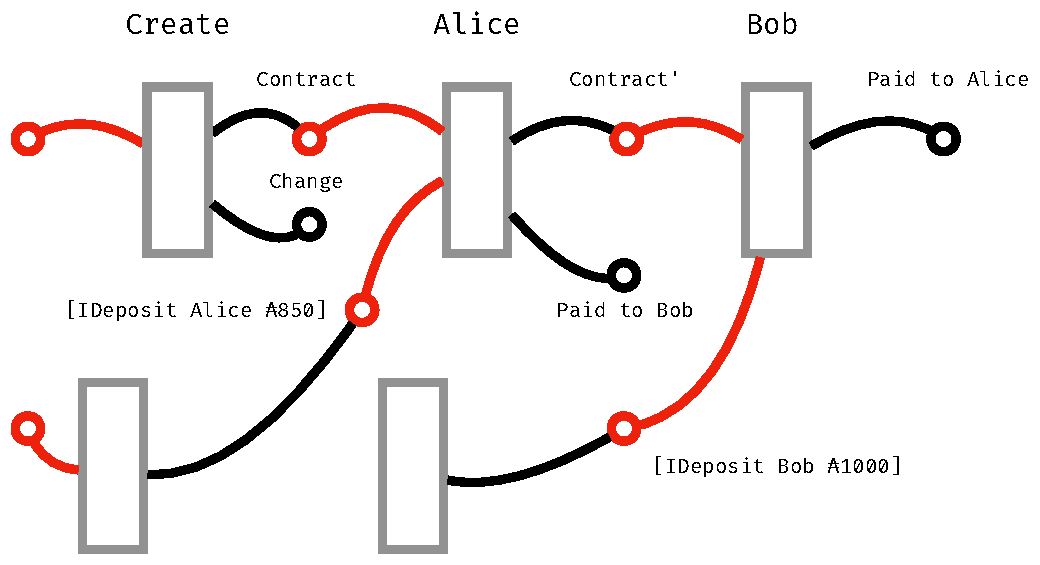
\includegraphics[width=4in]{figures/Marlowe3-Figure-2-crop.pdf}
    \caption{Zero Coupon Bond Contract}
    \label{fig:zero-coupon-bond}
\end{figure}

Note, that it is possible to provide multiple inputs at a time,
allowing as many steps of a contract execution as necessary to be merged.
This gives atomicity to some operations, and saves on transaction fees.

\paragraph{Ensuring execution validity}

Except for the transaction that closes a Marlowe contract, the Marlowe validator script checks that a spending transaction contains a valid continuation
output, i.e: the hash of the output validator is the same (same hash), and the new state and contract are the expected ones: the ones resulting from applying the \texttt{computeTransaction} to the given inputs.

\paragraph{Closing a contract}

When a contract evaluates to \texttt{Close}, all remaining balances the accounts of the contract are payed out
to the respective owners of each account, and the contract is removed from the set of unspent transaction outputs.

\subsection{Further Work}

Cardano extends its ledger rules to support \emph{forging} of custom currencies and tokens,
effectively embedding support of Ethereum ERC-20 and ERC-721 contracts. 
Simple token creation gives interesting possibilities of representing Marlowe contract parties by tokens.
This tokenization of contract participants abstracts away concrete public keys into contract \emph{roles}.
In turn, those roles could be traded independently of a contract.

We are working on adding \emph{multicurrency} or \emph{roles} support to Marlowe.

\section{Static analysis of contracts\label{sec:static}}

Marlowe semantics use types to prevent many non-sensical contracts from being written. But there are potential problems which are harder to detect until runtime, for example, whether there will be enough money to issue all the payments declared in the contract. At that point, it may already be too late to fix them, particularly in the case of blockchain.

Fortunately, in the case of Marlowe, a computer can decidedly determine whether a particular contract satisfies certain property before executing it, and it can provide a counter-example when it does not.

Our implementation relies on the Haskell library SBV, which in turn relies on existing SMT solvers to check satisfiability of properties.

\subsection{SBV library}

SBV \cite{SBV} (SMT Based Verification) library provides a high-level API that allows developers to automatically prove properties about Haskell programs, among other functionalities.
The SBV library translates these properties to SMTLib queries, passes them to one or several SMT solvers, and translates the results back to the format in which the queries were written.

\subsubsection{\texttt{SBV} monad}

SBV provides a monad called \texttt{SBV}, a function can use parameters wrapped in this monad to represent symbolic values. Functions that take symbolic values can be used as properties and passed to the solver, which will replace the symbolic values with concrete values that satisfy or falsify the property.

\subsection{Using SBV to analyse Marlowe Contracts}

Marlowe semantics represents errors that can be found at runtime as \texttt{Warnings}.

The property that we have implemented using SBV library can be enunciated as: ``the given contract will not need to issue warnings at runtime no matter the inputs it receives''.

This property is essentially a symbolic version of the semantics that returns a list of the warnings produced by a symbolic trace (a symbolic list of transactions input to the contract):

\begin{verbatim}
warningsTraceWB :: Bounds -> SSlotNumber -> SList NTransaction
                -> Contract -> SList NTransactionWarning
\end{verbatim}

\noindent
where types that begin with \texttt{S}, like \texttt{SSlotNumber}, are abbreviations for the symbolic versions of types: in this case \texttt{SBV SlotNumber}.
The types that begin with \texttt{N} are \textit{nested} types, which we explain in the \textit{Custom datatypes} section below.

\subsubsection{Custom datatypes}

SBV does not currently seem to support in general the use of custom datatypes. Fortunately, SBV supports tuples and the \texttt{Either} type. We can represent all types that Marlowe requires as combinations of \texttt{Either} and tuples, with the exception of the \texttt{Contract} type, but we do not need a symbolic version of the \texttt{Contract} type because we know its value at the time of analysis.

\noindent
For example, the \texttt{TransactionResult} type:
\begin{verbatim}
data TransactionResult
 = TransactionProcessed [TransactionWarning]
                        [TransactionEffect]
                        State
 | TransactionError TransactionError
\end{verbatim}
\noindent
becomes the nested type synonym \texttt{NTransactionResult}:

\begin{verbatim}
type NTransactionResult =
  Either ([NTransactionWarning], [NTransactionEffect], NState)
         NTransactionError
\end{verbatim}

\noindent
Because working with nested types is much more error prone than working with the original data-types, we used Template Haskell \cite{sheard2002template} to implement functions that transform the custom datatypes into nested types and generate the appropriate conversion functions.

\subsubsection{Bounds for the state and the inputs}

The recursion in the execution of the semantics is bounded by the \texttt{Contract}, and because the \texttt{Contract} is not a symbolic parameter, the translation will terminate.

However, in both the input and the \texttt{State} record there are several lists (representing finite maps) that are not explicitly bounded in the implementation. Some parts of the semantics are bounded by the length of these lists (or maps), such as the implementation of \texttt{Close}.
In order for the symbolic implementation to be finite, we need to find a bound for the length of these lists or maps.

Fortunately, we can infer a bound for all this lists quite straightforwardly. The least obvious one is the length of the list of transactions; we discuss the proof for this bound in Section~\ref{subsubsec:bound_max_transaction_number}.

\subsubsection{Returning non-symbolic \texttt{Contract} values}

Values that rely on symbolic values have to be themselves symbolic, and the continuation \texttt{Contract} after each step depends on the \texttt{Input}s and \texttt{State}, which are both symbolic. But having the contract as a symbolic parameter would be inconvenient since it is recursive, we know it in advance, and we use it to bound the execution of the symbolic semantics.

We work around this problem by modifying the signature of the function to receive a \textit{continuation function} instead, and instead of just returning a value, we return the result of applying the \textit{continuation function} to the result we were planning to return.

For example, the original type signature for the \texttt{apply} function was:

\begin{verbatim}
apply :: Environment -> State -> Input -> Contract -> ApplyResult
\end{verbatim}

\noindent
and the symbolic version of the \texttt{apply} function has the following signature:

\begin{verbatim}
apply :: SymVal a => Bounds
      -> SEnvironment -> SState -> SInput -> Contract
      -> (SApplyResult -> DetApplyResult -> SBV a) -> SBV a
\end{verbatim}

\noindent
where \texttt{DetApplyResult} contains the parts of \texttt{ApplyResult} that are not symbolic (like the \texttt{Contract}).

\section{Formal verification of the Marlowe semantics\label{sec:verification}}

We can also use proof assistants to demonstrate that the Marlowe semantics presents certain desirable properties, such as that money is preserved and anything unspent is returned to users by the end of the execution of any contract.

Currently, we have translated the Haskell Marlowe semantics to Isabelle while keeping both versions as close as possible, but we decided to make them different in two main aspects:

\begin{itemize}
    \item We use \emph{integers for identifiers} because they are easier to handle than strings.
    \item We use a \emph{custom implementation of maps and sets} that use lists because Isabelle already provides many theorems that are proved for lists.
\end{itemize}

\subsection{Termination proof}

Isabelle automatically proves termination for most function. This is not the case for \texttt{reductionLoop}. This function repeatedly calls \texttt{reduceContractStep} until it returns \texttt{NotReduced}, so proving overall termination requires a proof that \texttt{reduceContractStep} will eventually do that. In order to prove this, we defined a measure for the size of a pair of \texttt{Contract} and \texttt{State}:

\begin{verbatim}
fun evalBound :: "State ⇒ Contract ⇒ nat" where
"evalBound sta cont = length (accounts sta) + 2 * (size cont)"
\end{verbatim}
\noindent
where \texttt{size} is a measure already generated automatically by Isabelle.

We need the number of accounts in the \texttt{State} because the size of the contract \texttt{Close} will not decrease when calling \texttt{reduceContractStep}, but the number of accounts will, unless they are all empty.

And we needed to multiply the size of the \texttt{Contract} by two because the primitive \texttt{Deposit} may increase the number of accounts by one, so we need to multiply the effect of the reduction of the size of the contract in order to compensate that.

\subsection{Valid state and positive account preservation\label{subsec:valid_state}}

There are some values for \texttt{State} that are allowed by its type but make no sense, especially in the case of Isabelle semantics where we use lists instead of maps:

\begin{enumerate}
    \item The lists represent maps, so they should have no repeated keys.
    \item We want two maps that are equal to be represented the same, so we force keys to be in ascending order.
    \item We only want to record those accounts that contain a positive amount.
\end{enumerate}
\noindent
We call a value for \texttt{State} \emph{valid} if the first two properties are true. And we say it has \emph{positive accounts} if the third property is true.

We have proved that functions in the semantics preserve all three properties.

\subsubsection{Quiescent result}

A contract is \emph{quiescent} if and only if the root construct \texttt{When}, or if the contract is \texttt{Close} and all accounts are empty. We have proved that, if an input \texttt{State} is valid and accounts are positive, then the output will be quiescent.

\subsection{Money preservation and contract timeout}

One of the dangers of using smart contracts is that a badly written one can potentially lock its funds forever. By the end of the contract, all the money paid to the contract must be distributed back, in some way, to a subset of the participants of the contract.
To ensure this is the case we proved two properties:

\subsubsection{Money preservation}
Money is not created or destroyed by the semantics. More specifically, the money that comes in plus the money in the contract before the transaction must be equal to the money that comes out plus the contract after the transaction, except in the case of an error.

\subsubsection{Timeout closes a contract}

For every Marlowe \texttt{Contract} there is a slot number after which an empty transaction can be issued that will close the contract and refund all the money in its accounts.

A conservative upper bound for the expiration slot number can be calculated efficiently by using the function \texttt{maxTime} (or \texttt{maxTimeContract} in the Isabelle semantics), essentially by taking the maximum of all the timeouts in the contract.

We proved that this conservative upper bound is general enough for every contract, by showing that, if the contract is not closed and empty, then an empty transaction sent after \texttt{maxTime} will close the contract and empty the accounts.

\subsection{Bound on the maximum number of transactions\label{subsubsec:bound_max_transaction_number}}

Another property of Marlowe is that any given finite \texttt{Contract} has an implicit finite bound on the maximum number of \texttt{Transaction}s that it accepts. This is a convenient property because:

\begin{itemize}
    \item It reduces the danger of Denial of Service (DoS) attacks: because the number of valid inputs is limited, an attacker participant cannot arbitrarily block the contract by issuing an unbounded amount of useless \texttt{Transaction}s.
    \item The number of transactions bounds the length of traces that symbolic execution (see Section~\ref{sec:static}) needs to explore (more on this below).%SJT: is this really below? Or above?
\end{itemize}

We state the property as follows:

\begin{verbatim}
lemma playTrace_only_accepts_maxTransactionsInitialState :
"playTrace sl c l = TransactionOutput txOut
  ⟹ length l ≤ maxTransactionsInitialState c"
\end{verbatim}

\noindent
where \texttt{maxTransactionsInitialState} is essentially the maximum number of nested \texttt{When} constructs in the contract plus one.

This property implies that any trace that is longer than this is guaranteed to produce at least one error. Because transactions that produce an error do not alter the state of the contract, such a list of transactions (a trace) will be equivalent to a list of transactions that does not have the erroneous transaction.
Thus, we do not lose generality by only exploring shorter traces.

\section{The Marlowe Playground}
\label{sec:playground}

For Marlowe to be usable in practice, users need to be able to design and develop Marlowe contracts, and also to understand how contracts will behave once deployed to the blockchain, but without actually deploying them.

The Marlowe Playground, a web-based tool that supports the interactive construction, revision, and simulation of smart contracts written in Marlowe, provides these facilities, as well as access to a static analysis of contracts (as described in the previous section), an online tutorial for Marlowe and a set of example contracts. The playground is available at \url{https://prod.meadow.marlowe.iohkdev.io/}.\footnote{Development of the playground is rapid, and the latest, unstable, version is also available at \url{https://alpha.marlowe.iohkdev.io/}.}

At the top level, the playground offers three panes: the main \emph{Simulation} pane, as well as panes for developing Marlowe contracts, embedded in \emph{Haskell} or using the \emph{Blockly} visual language.

\paragraph{Development}

On the simulation pane, ``pure'' Marlowe contacts can be developed directly, not embedded in another language. Two reasons for doing this are:
\begin{itemize}
    \item There is a shallower learning curve for users who are new to Haskell or programming languages in general. The Marlowe constructs are quite simple, and there is no need, at least initially, to learn about Haskell syntax or even variables, functions etc.
    \item As we step through the execution of a contract in a simulation, the contract is reduced; it is very useful to be able to view, or even edit, the reduced contract during this execution.
\end{itemize}
As contracts become larger it makes sense to use another editor in the \emph{Haskell} pane. Here contracts can be written using facilities from \emph{Haskell} to abbreviate and make more readable the description of the contracts. These contracts can then be transferred as a pure Marlowe data structure into the simulation pane.

Contracts can also be written using Google's \emph{Blockly} visual programming language, as was earlier described in Meadow~\cite{isola-marlowe}. Blockly gives an easy way to introduce the concepts of Marlowe to users who have no programming knowledge, and in particular the editor gives users a set of options for each construct as the contract is built. Once a contract has been constructed in Blockly it is possible to transfer that contract to the simulation pane. It is also possible to transfer a Marlowe contract to Blockly for further editing.

\begin{wrapfigure}[9]{l}{0.25\textwidth}
    \vspace*{-0.28in}
    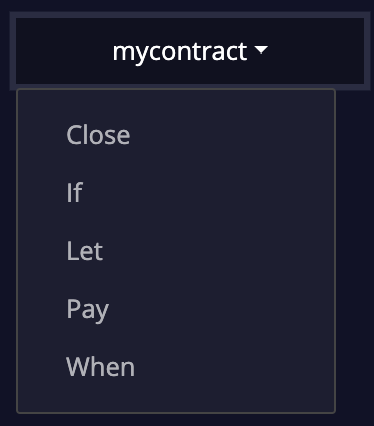
\includegraphics[width=0.25\textwidth]{hole_options.png}
\end{wrapfigure}

The Marlowe editor in the unstable version of the playground has a feature called \emph{holes} to aid writing contracts. If we enter the contract \lstinline{?mycontract}
%SJT: enter it where?
we will be presented with a dropdown list of values that could be used.

In our case \lstinline{?mycontract} must be a \lstinline{Contract} of some sort, and so we are offered a choice of \lstinline{Contract} constructors from a dropdown list. If we choose \lstinline{Pay} then the Marlowe editor will automatically fill in a skeleton \lstinline{Pay} contract with new holes where we need to provide values.
\begin{verbatim}
    Pay ?accountId_1_1 ?payee_1_2 ?value_1_3 ?contract_1_4
\end{verbatim}
New options will be presented, one for each hole, and each will have a dropdown list of all the possible values.

\begin{wrapfigure}[6]{l}{0.25\textwidth}
    \vspace*{-0.00in}
    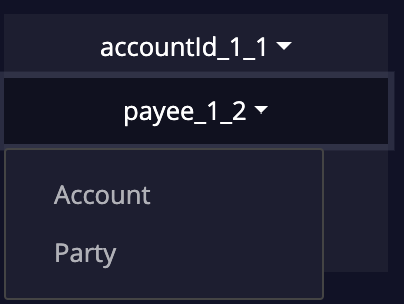
\includegraphics[scale=0.2]{hole_options_2.png}
\end{wrapfigure}
A complete contract can be written in this guided way with the user needing only to fill in strings and numbers by hand. This approach to writing holes in your code and ``asking'' the compiler what you could put in there is easy to implement in a DSL because there are very limited options, however is is also becoming popular with more complex languages such as Haskell and Idris.

Users can at any point save the current contract directly to a Github Gist, as well as being able to re-load contracts from Github Gists. There are also some demo contracts that can be loaded in their Haskell and Marlowe versions.

\paragraph{Simulation}

Contracts written in the Marlowe editor are parsed in real-time and if there are no errors (and no holes) then the contract is analysed to discover which actions a user could take to progress the contract. These actions are displayed in the ``Input Composer'' above the editor. Consider the following example contract:
\begin{verbatim}
    When [Case (Deposit (AccountId 0 "investor") 
               "guarantor" (Constant 1000_000000)) Close] 10 Close
\end{verbatim}
In this case, the only action a user can take to progress the contract is to accept a deposit of 1000 ADA
from the guarantor to the investor's account. Because of this, the playground can display this action in the input composer.

\begin{wrapfigure}[5]{l}{0.5\textwidth}
    \vspace*{-0.2in}
    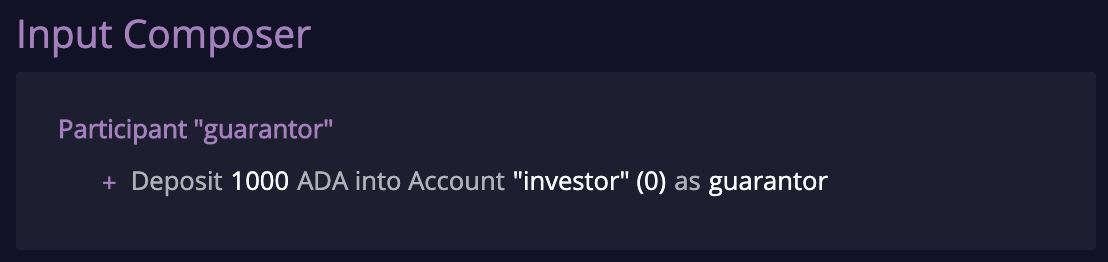
\includegraphics[scale=0.15]{input_composer.png}
\end{wrapfigure}

\noindent
The user can then choose to add this action to a transaction being prepared. Once the action is added other inputs become possible; these are displayed in the input composer, and again they can be added to the transaction being composed. In this way, multiple actions can be added to a transaction before it is applied.

\begin{wrapfigure}[6]{l}{0.5\textwidth}
    \vspace*{-0.2in}
    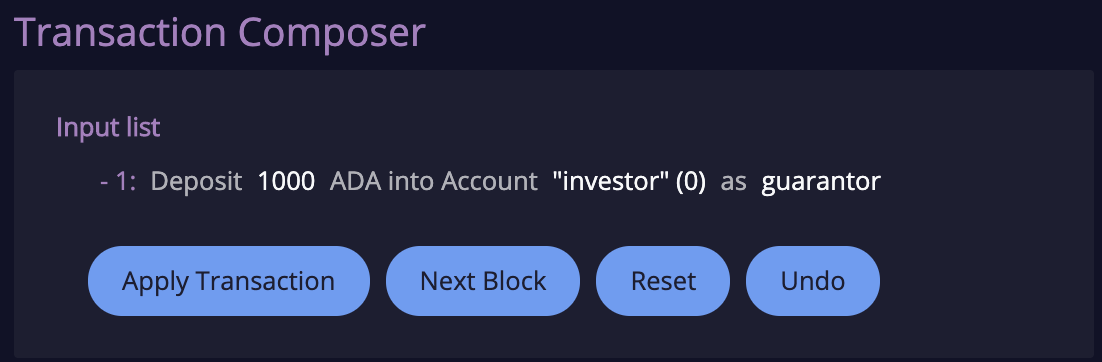
\includegraphics[scale=0.15]{tx_composer.png}
\end{wrapfigure}

\noindent
A user can then apply this transaction and in the example above this would result in the state pane showing a single payment and in addition the contract in the Marlowe editor will have been reduced to \lstinline{Close}.

At any point in the simulation, the user can undo any steps made: in this particular case, they can undo the application of the transaction, and iteratively undo more steps. At any point, they can also reset the contract to its initial state. This enables users to apply transactions, see their effects, step back, and try different transactions to see the effects of the changes on the result. They can also change the reduced contract to investigate variants of the original.

The final feature that we would like to present is the static analysis of contracts. As described in the previous section, it is possible to carry out a symbolic execution of a contract and then use a SMT solver to look for cases that could cause unwanted situations. The playground uses this to search for situations where contract execution would cause warnings. For example, suppose you write a contract that causes a payment of 450 Lovelace from Alice to Bob but the contract allows a situation where Alice has only deposited 350 Lovelace. The the static analysis will find this partial payment case and report it to the playground user with an example of how it could occur.

\section{Related work}
\label{sec:related}

An earlier paper~\cite{cryptoeprint:2016:1156} reviews smart contracts on blockchain. Here we look at a number of recent systems that bear direct comparison with Marlowe.

The Ethereum system~\cite{wood2014ethereum} provides an exemplar Turing-complete language for  the EVM virtual machine, and a higher-level programming language, Solidity, that compiles into EVM code. Both these languages are general-purpose, and so have more akin with Plutus~\cite{PlutusPlatform} rather than Marlowe.

On the other hand,  Nxt~\cite{Nxt}, is special-purpose in providing a ``fat'' high-level
API, containing built-in transaction types and transactions that support some 250 primitive operations; these can be ``scripted'' in a client (only) using a binding to the API, which is available, for instance, in JavaScript. In providing such specificity this bears comparison with our implementation of contracts from the ACTUS standard~\cite{actus}.

Our work is inspired by the original work of Peyton Jones and others~\cite{PeytonJones:2000} to describe financial contracts using a DSL embedded in Haskell. The Findel project~\cite{findel} examines financial contracts on the Ethereum platform, and is also based on~\cite{PeytonJones:2000}. The authors note that payments need to be bounded; this is made concrete in our
account by our notion of commitments. They take no account of commitments or timeouts as our approach does, and so are unable to guarantee some of the properties -- such as a finite lifetime -- built into Marlowe by design.

BitML~\cite{BitML} is a DSL for specifying Marlowe-like contracts that regulate transfers on the Bitcoin blockchain. BitML is implemented via a compiler that translates contracts into standard Bitcoin transactions. Participants execute a contract by appending these transactions on the Bitcoin blockchain, according to their strategies, which also involve the exchange of bitstrings that guarantee to a very high probability the correctness of contract execution. Marlowe is directly implemented by an interpreter which could also be implemented on a covenant-based~\cite{covenants} extension of the Bitcoin blockchain.

\section{Conclusions and future work}

Rather than aiming to be general-purpose, Marlowe is a DSL designed to support financial contracts on blockchain. We leverage its specificity in our work on static analysis and verification, where we are able to deliver much greater impact and focus than we could for a general-purpose language. We are able to shape the development and simulation environment to give stronger user support too. Moreover, Marlowe  presents a model for how other DSLs can be built in this space, supporting different domains such as provenance in the supply chain. 

Defining the language by means of an executable reference semantics means that we can, as well as directly executing this semantics, generate an on-chain interpreter for it and simulate it in browser using the Haskell-like languages Plutus and PureScript. This is particularly straightforward when working with a subset of Haskell that is represented in the same way on these languages.

Our medium term aim is launching on Cardano blockchain itself, by which time we expect to have added multiple currencies to Marlowe, as well as making (roles in) Marlowe contracts tradeable, through tokenising contract roles.


%
% ---- Bibliography ----
%
% BibTeX users should specify bibliography style 'splncs04'.
% References will then be sorted and formatted in the correct style.
%
\bibliographystyle{splncs04}
\bibliography{paper}
%
\end{document}
